\section{Differentialgleichungen \formelbuch{543}}

\subsection{L"osen von Differentialgleichungen}

\subsubsection{Trennung von Variabeln / Separation \formelbuch{545}}
\begin{tabular}{p{4cm}p{1.5cm}p{10.5cm}}
\textbf{Form:} $y' = f(x) g(y)$ &
\textbf{Vorgehen:}              &
1. DGL umstellen: $\frac{y'}{g(y)} = f(x)$ \\ &&
2. Beidseitig nach x integrieren wobei $dx = \frac{dy}{y'}$ \\ &&
3. Genzen anpassen: $\int_{y_0=y(x_0)}^{y} \frac{1}{g(y)} dy =
\int_{x}^{x_0}f(x) dx$
\end{tabular}

\subsubsection{Lineartermsubstitution \formelbuch{545}}
\begin{tabular}{p{4cm}p{1.5cm}p{10.5cm}}
\textbf{Form:} $y'=f(ax+by+c)$   &
\textbf{Vorgehen:}               &
1. Substitution: $z=ax+by+c$ \\ &&
3. Einsetzen in $z'=a+bf(z)$\\ &&
2. Separation: $\frac{z'}{f(z)} = a + b$ wobei $z_0 = x_0 + y_0$
\end{tabular}

\subsubsection{Gleichgradigkeit}
\begin{tabular}{p{4cm}p{1.5cm}p{10.5cm}}
\textbf{Form:} $y'=f(\frac{y}{x})$ &
\textbf{Vorgehen:}                &
1. Substitution:\quad $z=\frac{y}{x}$\\ &&
2. Einsetzen in $z'=\frac{1}{x}(f(z)-z)$\\ &&
3. Seperation: $\frac{z'}{f(z)-z} = \frac{1}{x}$ wobei $z_0 = \frac{y_0}{x_0}$ 
\end{tabular}

\subsubsection{Lineare Differentialgleichungen 1. Ordnung \formelbuch{546}}
\begin{tabular}{p{4cm}p{1.5cm}p{10.5cm}}
\textbf{Form:} $ y'+f(x)y = g(x) $ &
\textbf{Vorgehen:}                 &
Homogene Rechunug: $y_H = k \cdot e^{-\int f(x) \cdot dx}$\\ &&
Inhomogene Rechunug: $y_P = (\int g(x) \cdot e^{\int f(x) \cdot dx} \cdot dx)
\cdot e^{-\int f(x) \cdot dx}$\\ &&
Allgemeine Lösung: $y = y_H + y_P$ wobei $k = \frac{y_0 - y_P(x_0)}{e^{\int
f(x_0) \cdot dx)}}$
\end{tabular}

\subsection{Lineare Differentialgleichung 2. Ordnung mit konstanten 
Koeffizienten \formelbuch{564}}
\begin{tabular}{p{8cm}p{8cm}}
\textbf{Form:} $y''+a_1\cdot y'+a_0\cdot y=f(x)$  &
\textbf{St"orglied:} $f(x)$\\
\textbf{Homogene Differentialgleichung:} $f(x)=0$ &
\textbf{Inhomogene Differentialgleichung:} $f(x)\neq 0$
\end{tabular}

\subsubsection{Homogene L"osung $y_H$}
\begin{tabular}{p{8cm}p{8cm}}
\textbf{Charakteristisches Polynom:} \newline
$\qquad\lambda^2+a_1\cdot\lambda+a_0=0$ \quad
$\lambda_{1,2} = -\frac{a_1}{2} \pm \sqrt{\frac{{a_1}^2}{4}-a_0}$ &
\textbf{Diskriminante:} \newline
$D = \frac{{a_1}^2}{4}-a_0$ 
\end{tabular} \\ \\

\begin{tabular}{p{4cm}p{12cm}}
Falls $D > 0$:&
$y_H=A_1e^{\lambda_1x}+A_2e^{\lambda_2x}$\\
Falls $D = 0$:&
$y_H=e^{\lambda_1x}(A_1+A_2\cdot x)$\\
Falls $D < 0$:&
$y_H=e^{-\frac{1}{2}a_1x}(A_1 \cdot cos(\sqrt{|D|} x) +A_2 \cdot sin(\sqrt{|D|}
x))$
\end{tabular}

\subsubsection{Partikuläre Lösung $y_P$ durch Faltung}
$y_P(x)=\int\limits_{x_o}^{x} g(x+x_0-t) \cdot f(t) \cdot dt$ \\

$g(x)$ entspricht $y_H$ mit Standartanfang $g(x_0) = 0, g'(x_0)
= 1$ (womit die Freiheitsgrade $A_1$ und $A_2$ bestimmt werden)

\subsubsection{Partikuläre Lösung $y_P$ durch Form des Störglieds $f(x)$}
 ($p_n(x) = \sum_{k=1}^{n}\alpha_k x^k$,
$q_n(x)=\sum_{k=1}^{n} \beta_k x^k$, $r_n=\ldots$ und $s_n=\ldots$ sind Polynome vom
n. Grad)\\ \\
\textbf{Allgemeines Vorgehen:}\\
1. Ermitteltes $y_P$ n mal ableiten \\
2. Ableitungen in DGL einsetzen \\
3. Koeffizientenvergleich \\ \\
\underline{$f(x)=p_n(x)$}\\
\begin{tabular}{p{8cm}p{4cm}}
$a_0\neq 0$:          & $y_P = q_n(x)$\\
$a_0 = 0 , a_1\neq 0$:& $y_P=x\cdot q_n(x)$\\
$a_0=a_1=0$:          & $y_P=x^2\cdot q_n(x)$\\
\end{tabular}\\ \\ \\
\begin{tabular}{p{2cm}p{10cm}}
$x^n$: & $\beta_n = \frac{\alpha_n}{a_0}$ \\ 
$x^{n-1}$: & $\beta_{n-1} = \frac{1}{a_0}(\alpha_{n-1} - a_1\beta_n \cdot n)$ \\
$x^k$: & $\alpha_k = \beta_{k+2}(k+2)(k+1)+a_1 \cdot \beta_{k+1} \cdot (k + 1) +
a_0 \cdot \beta_k $ (für $0 \leqq k \leqq n-2 $)
\end{tabular} \\ \\

\underline{$f(x)=e^{bx}\cdot p_n(x)$} \\
\begin{tabular}{p{8cm}p{4cm}}
Fall a: $b$ nicht Nullstelle des char. Polynoms:    &
$y_P=e^{bx}\cdot q_n(x)$\\
Fall b: $b$ einfache Nullstelle des char. Polynoms: &
$y_P=e^{bx}\cdot x \cdot q_n(x)$\\
Fall c: $b$ zweifache Nullstelle des char. Polynoms: &
$y_P=e^{bx}\cdot x^2\cdot q_n(x)$
\end{tabular}\\ \\ \\
\begin{tabular}{p{2cm}p{9cm}}
$x^n e^{bx}$: & $\beta_n = \frac{\alpha_n}{(2b+a_1)(n+1)}$ \\
$x^k e^{bx}$: & $\beta_k = \frac{\alpha_k - \beta_{k+1} \cdot (k+2)(k+1)}{(2b+a_1)(k+1)}$
\end{tabular} \\ \\

\underline{$f(x)=e^{cx}(p_n(x)\cos{bx}+q_n(x)\sin{bx})$}\\
\begin{tabular}{p{8cm}p{8cm}}
Fall a: $c+jb$ \textbf{nicht} Lösung der char. Gleichung &
$y_p=e^{cx}(r_n(x)\cos{bx}+s_n(x)\sin{bx})$ \\
Fall b: $c+jb$ Lösung der char. Gleichung &
$y_p=e^{cx}x(r_n(x)\cos{bx}+s_n(x)\sin{bx})$\\
\end{tabular}\\

\subsubsection{Partikuläre Lösung durch Superpositionsprinzip}
$f(x)=c_1f_1(x)+c_2f_2(x)$\\
\begin{tabular}{p{8cm}p{4cm}}
$y_1$ ist spezielle L"osung der DGL &
$y''+a_1\cdot y'+a_0\cdot y=c_1f_1(x)$ \\
$y_2$ ist spezielle L"osung der DGL &
$y''+a_1\cdot y'+a_0\cdot y=c_2f_2(x)$ \\
dann ist:                          &
$y_P=c_1y_1+c_2y_2$\\
\end{tabular}

\subsubsection{Allgemeine L"osung einer DGL}
$Y=y_H+y_P$

\subsection{Lineare Differentialgleichung n. Ordnung mit konstanten 
Koeffizienten \formelbuch{554}}
\begin{tabular}{p{8cm}p{8cm}}
\textbf{Form:} &
$\sum\limits_{k=0}^na_ky^{(k)}= y^{(n)}+a_{n-1}\cdot y^{(n-1)}+\ldots +a_0\cdot y=f(x)$\\
\textbf{Algemeine L"osung der homogenen DGL:} &
$g=c_1g_1+c_2g_2+\ldots +c_kg_k$\\
\end{tabular}

\subsubsection{Homogene L"osungen}
\begin{tabular}{lll}
Fall a: r reelle L"osungen $\lambda_1$: 
  & $y_1=e^{\lambda_1x}$, $y_2=xe^{\lambda_1x}$, \ldots
  ,$y_r=x^{r-1}e^{\lambda_1x}$ 
  & Starke D"ampfung / Kriechfall\\
Fall b: $k$ komplexe L"osungen $\lambda_2=\alpha +j\beta$: 
  &$y_1=e^{\alpha x}\cos(\beta x)$, \ldots, $y_k=e^{\alpha x}x^{k-1}\cos(\beta
x)$
  & Schwache D"ampfung /\\
  &$y_{k+1}=e^{\alpha x}\sin(\beta x)$, \ldots, $y_{2k}=e^{\alpha
x}x^{k-1}\sin(\beta x)$
  & Schwingfall\\
\end{tabular}

\subsubsection{Allgemeinste L"osung des partikul"aren Teils:}
$$\underbrace{\sum_{k=0}^n a_k y^{(k)}}_{f(y,y',y'',\ldots)} = \underbrace{e^{\alpha x} (p_{m1}(x) \cos (\beta x) + q_{m2}(x) \sin (\beta x))}_{\text{St"orglied}}$$
Unterscheide die L"osungen des charakteristischen Polynoms
($\lambda$):\hspace{5.5cm}mit m = max(m1, m2)\\
\begin{tabular}{p{8cm}p{8.5cm}}
Fall a: $\alpha + j\beta \neq \lambda$, so ist &
$y_P = e^{\alpha x}(r_m(x)\cos(\beta x) + s_m(x) \sin(\beta x))$\\
Fall b: $\alpha + j\beta$  ist u-fache L"osung von $\lambda$, so ist &
$y_P = e^{\alpha x} x^u (r_m(x) \cos(\beta x) + s_m(x) \sin(\beta x))$\\
&
u-fache Resonanz

\end{tabular}

\subsubsection{Grundl"oseverfahren}
\begin{tabular}{p{12cm}p{5cm}}
$\begin{pmatrix}
g(x_0)=  & 0 & = & c_1g_1(x_0)+c_2g_2(x_0)+\ldots +c_n(x_0)\\
g'(x_0)= & 0 & = & c_1g_1'(x_0)+c_2g_2'(x_0)+\ldots +c_ng_n'(x_0)\\
\vdots  & \vdots & \\                            
g^{(n-1)}(x_0)= & 1 & = & c_1g_1^{(n-1)}(x_0)+c_2g_2^{(n-1)}(x_0)+\ldots
+c_ng_n^{(n-1)}(x_0)
\end{pmatrix}$ &
\begin{minipage}[t]{5cm}
ergibt $c_1,\ldots ,c_n$ f"ur\\
$y_{P}(x)=\int_{x_0}^x{g(x+x_0-t)f(t)dt}$
\end{minipage}
\end{tabular}

\subsubsection{Hornerschema\formelbuch{914}}
\begin{minipage}[t]{9cm}
- Pfeile $\Rightarrow$ Multiplikation\\
- Zahlen pro Spalte werden addiert\\
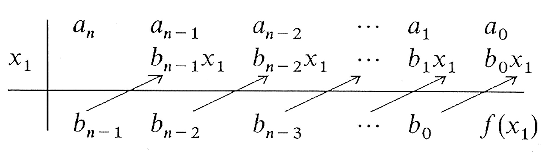
\includegraphics[width=6cm]{./bilder/Hornerschema_1.png}\\
$x_1 \Rightarrow$ Nullstelle (muss erraten werden!!)\\
oberste Zeile = zu zerlegendes Polynom
\end{minipage}
\begin{minipage}[t]{9cm}
\textbf{Beispiel:}\\
$f(x) = x^3-67x-126$\\
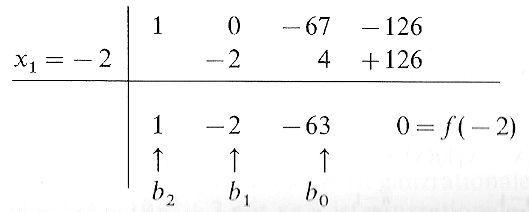
\includegraphics[width=6cm]{./bilder/Hornerschema_2.png}\\
$\Rightarrow f(x) = (x-x_1)(b_2x^2 + b_1x + b_0) = (x+2)(x^2-2x-63)$  
\end{minipage}

\subsection{Lineare Differentialgleichungssysteme erster Ordnung mit konstanten
Koeffizienten}
\begin{tabular}{p{8cm}p{8cm}}
\textbf{Form:}&
$\dot{x}=ax+by+f(t)$\\
&
$\dot{y}=cx+dy+g(t)$\\
\textbf{Die allgem. L"osung ergibt sich aus der DGL:}&
$\ddot{x}-(a+d)\dot{x}+(ad-bc)x=\dot{f}(t)-d \cdot f(t)+b \cdot g(t)$\\
&
$y=\frac{1}{b}(\dot{x}-ax-f(t)))$\\
\end{tabular}

\subsection{D"ampfung}
\begin{itemize}
  \setlength{\itemsep}{1pt}
  \setlength{\parskip}{0pt}
  \setlength{\parsep}{0pt}
  
  \item Starke Dämpfung: $D>0$
  \item Grenzfall; $D=0$
  \item Schwingfall / schawache D"ampfung: $D<0$
\end{itemize}
Frequenz: $\omega = \frac{\sqrt{\left|D\right|}}{2}$
Dämpfung $\left|\delta\right| = \left|{\frac{a_1}{2}}\right|$
siehe: $\lambda_{1,2}= -\frac{a_1}{2}\pm \frac{\sqrt{{a_1}^2-4a_0}}{2}$
